\section{Instrument control}\label{sec:control}

The new control framework has greatly improved the observing efficiency of the instrument, in some cases improving from $\sim$30\% to 95\% through asynchronous control. SCExAO uses multiple computers for real time control and computation to keep latency low. The cameras require dedicated resources because they can produce over \SI{20}{GB/s} each. The detectors are both connected to a data acquisition computer and integrated into the same high-speed streaming framework that is used for the SCExAO real-time control, enabling asynchronous file writing. Instrument metadata are managed with a \texttt{redis} database which combines facility status values with local SCExAO values and each camera's individaul attributes. Observing data are compressed and transferred nightly to the Subaru STARS2 archive.

The devices for controlling VAMPIRES (filter wheels, translation stages, etc.) are connected to their own dedicated computer with a python and command-line interface which can be accessed over the network from any SCExAO computer\footnote{\url{https://github.com/scexao-org/device_control}}. The VAMPIRES cameras each have custom \texttt{PyGame} viewers\footnote{\url{https://github.com/scexao-org/camstack}} which allow high-speed (\SI{30}{fps}) image display even during acquisition (\autoref{fig:vcam1}). Keyboard shortcuts are integrated for instrument control, facilitating alignment, focusing, filter switches, and more.

\begin{figure}
    \centering
    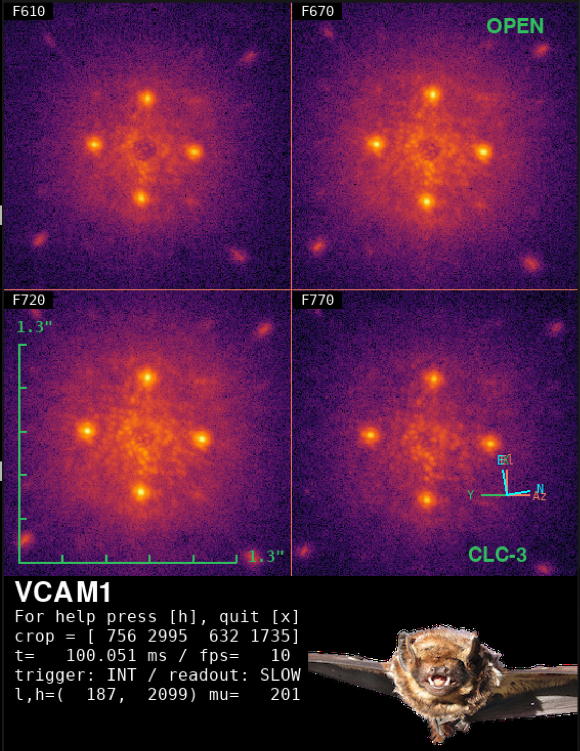
\includegraphics[width=0.95\columnwidth]{figures/vcam1_viewer.png}
    \caption{The custom \texttt{PyGame} camera viewer for VCAM1. Shown is a screenshot from on-sky observations on \formatdate{7}{7}{2023} in multiband imaging mode with the \SI{59}{\mas} coronagraph and 15.9$\lambda/D$ calibration speckles. The bat in the camera viewers is the endangered Hawai'ian Ope'ape'a.\label{fig:vcam1}}
\end{figure}
